\documentclass{article}
\usepackage[a4paper, total={7in, 10in}]{geometry}
\usepackage{graphicx} % Required for inserting images
\usepackage{listings}
\usepackage{float}

\title{Relatório do Lab 0 — Grupo 7}
\author{Eduardo Henrique Basilio de Carvalho \\
        Guilherme Alves Sousa \\
        Leonardo Reis Domingues Paes}
\date{Outubro 2024}

\begin{document}

\maketitle
\pagebreak

\begin{enumerate}
    \item Neste laboratório, usamos uma placa Arduino Uno R3. O programa foi desenvolvido no ambiente de desenvolvimento integrado da Arduino. A figura \ref{fig:esquematico} mostra as interfaces e conexões usadas.
    \begin{figure}[H]
        \centering
        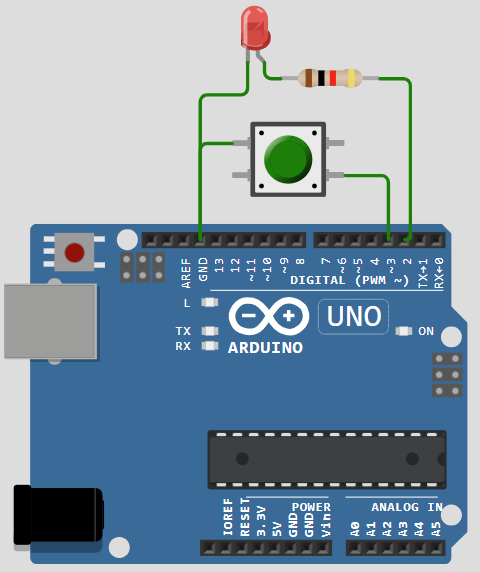
\includegraphics[width=0.5\linewidth]{esquematico.png}
        \caption{Esquemático do sistema}
        \label{fig:esquematico}
    \end{figure}

    \item O botão atua como chave entre o pino usado como entrada e a tensão de referência. Um resistor de \textit{pull-up} externo não é necessário porque a porta esta configurada para conectar este pino, internamente, a um. A conexão entre botão e placa é vista na figura \ref{fig:esquematico}.

    \item O anodo do LED está conectado a um resistor de 1 k\textohm e seu anodo está conectado à tensão de referência. O resistor está conectado ao pino usado como saída na placa. Pela forma como está conectado, o pino, quando em nível alto, fornece corrente ao LED.

    \item \ \\
\begin{lstlisting}[breaklines=true, language=C++]
// simulation: https://wokwi.com/projects/411926223458480129

const int ledPin = 2;
const int buttonPin = 3;
const int period = 2000;
const int blinkInterval = period / 2;
const int debounceTime = 100;
const int ledAckHighDuration = 250;

bool debounce(int pin, int interval, int stateToCheck);
void waitForButtonTobePressedandReleased(int buttonPin, int debounceTime, int pressedState = LOW);
void blinkLed(int ledPin, int interval);
void ackLed(int ledPin, int duration);

void setup()
{
  pinMode(ledPin, OUTPUT);
  pinMode(buttonPin, INPUT_PULLUP); // no need for external pull-up resistor
}

void loop()
{
  waitForButtonTobePressedandReleased(buttonPin, debounceTime);
  blinkLed(ledPin, blinkInterval);
  ackLed(ledPin, ledAckHighDuration);
}

bool debounce(int pin, int interval, int stateToCheck)
{
  if (digitalRead(pin) == stateToCheck) {
    delay(interval);
    if (digitalRead(pin) == stateToCheck) {
      return true;
    }
  }
  return false;
}

void waitForButtonTobePressedandReleased(int buttonPin, int debounceTime, int pressedState)
{
  int releasedState = not pressedState;

  while (!debounce(buttonPin, debounceTime, pressedState)) {
    // wait for the button to be pressed
  }

  while (!debounce(buttonPin, debounceTime, releasedState)) {
    // wait for the button to be released
  }
}

void blinkLed(int ledPin, int interval)
{
  int ledState = digitalRead(ledPin);

  digitalWrite(ledPin, not ledState);
  delay(interval);
  digitalWrite(ledPin, ledState);
  delay(interval);
}

void ackLed(int ledPin, int duration)
{
  int ledState = digitalRead(ledPin);

  digitalWrite(ledPin, not ledState);
  delay(duration);
  digitalWrite(ledPin, ledState);
}
\end{lstlisting}

    \item O experimento é simples e uma boa introdução aos laboratórios.
    
\end{enumerate}

\end{document}
